%%%%%%%%%%%%%%%%%%%%%%%%%%%%%%%%%%%%%%%%%%%%%%%%%%%%%%%%%%%%%%%%%%%%%%%%%%%%%%%%%%
\begin{frame}[fragile]\frametitle{}
\begin{center}
{\Large Theory}
\end{center}
\end{frame}

%%%%%%%%%%%%%%%%%%%%%%%%%%%%%%%%%%%%%%%%%%%%%%%%%%%%%%%%%%%%%%%%%%%%%%%%%%%%%%%%%%
\begin{frame}[fragile]\frametitle{Time Series Simple Example}
      \begin{center}
        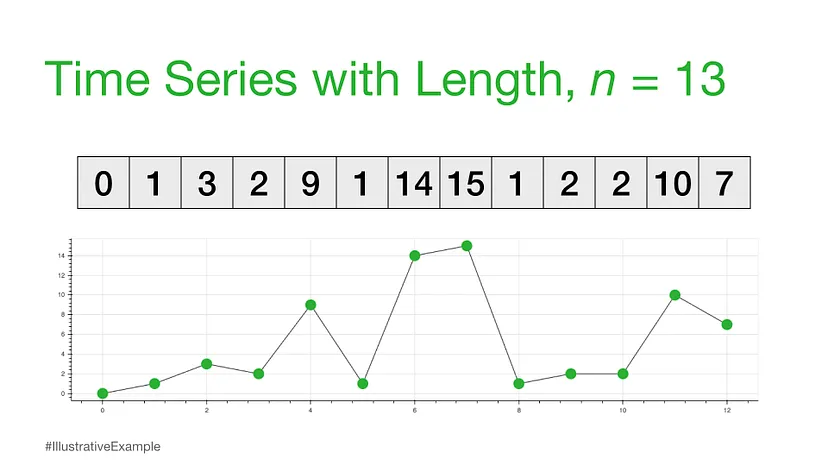
\includegraphics[width=0.8\linewidth,keepaspectratio]{timeseries1}

		{\tiny (Ref: Thomas J. Fan - Time Series EDA with STUMPY)}		
        \end{center}
	
\begin{lstlisting}
time_series = [0, 1, 3, 2, 9, 1, 14, 15, 1, 2, 2, 10, 7]
n = len(time_series)

n = 13
\end{lstlisting}	
\end{frame}

%%%%%%%%%%%%%%%%%%%%%%%%%%%%%%%%%%%%%%%%%%%%%%%%%%%%%%%%%%%%%%%%%%%%%%%%%%%%%%%%%%
\begin{frame}[fragile]\frametitle{Sub-sequence}

A continuous subset is a sub-sequence

      \begin{center}
        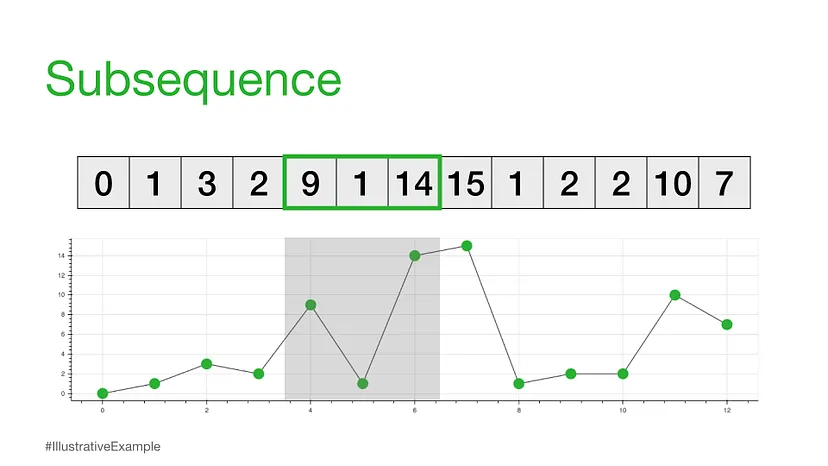
\includegraphics[width=0.8\linewidth,keepaspectratio]{timeseries2}

		{\tiny (Ref: Thomas J. Fan - Time Series EDA with STUMPY)}		
        \end{center}
	

\end{frame}

%%%%%%%%%%%%%%%%%%%%%%%%%%%%%%%%%%%%%%%%%%%%%%%%%%%%%%%%%%%%%%%%%%%%%%%%%%%%%%%%%%
\begin{frame}[fragile]\frametitle{Finding Patterns}

Compare all possible sub-sequences and find repeating ones, that's Pattern Detection.

      \begin{center}
        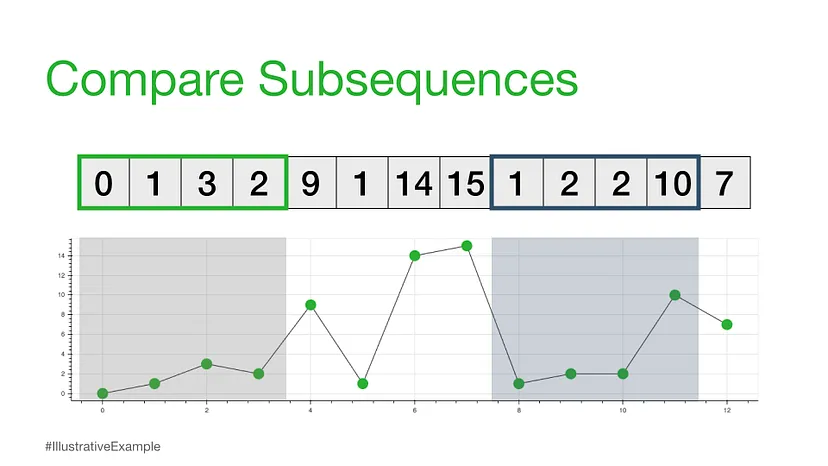
\includegraphics[width=0.8\linewidth,keepaspectratio]{timeseries3}

		{\tiny (Ref: Thomas J. Fan - Time Series EDA with STUMPY)}		
        \end{center}
	

\end{frame}

%%%%%%%%%%%%%%%%%%%%%%%%%%%%%%%%%%%%%%%%%%%%%%%%%%%%%%%%%%%%%%%%%%%%%%%%%%%%%%%%%%
\begin{frame}[fragile]\frametitle{How to Compare Sub-Sequences?}

Euclidean Distance

      \begin{center}
        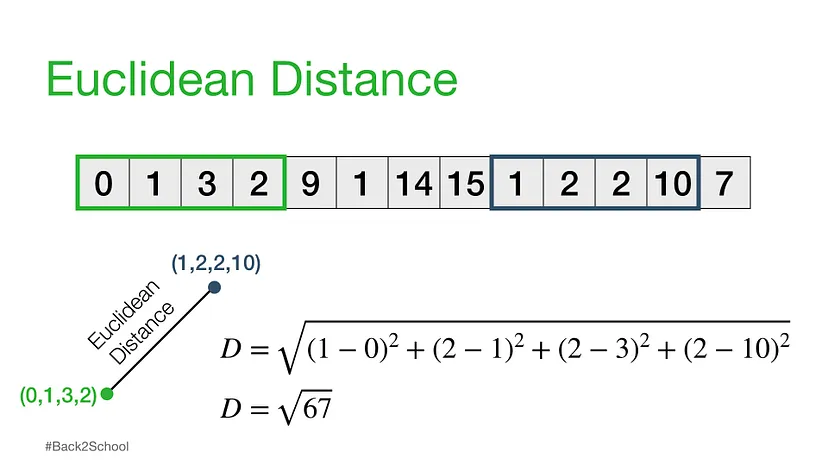
\includegraphics[width=0.8\linewidth,keepaspectratio]{timeseries4}

		{\tiny (Ref: Thomas J. Fan - Time Series EDA with STUMPY)}		
        \end{center}
	

\end{frame}

%%%%%%%%%%%%%%%%%%%%%%%%%%%%%%%%%%%%%%%%%%%%%%%%%%%%%%%%%%%%%%%%%%%%%%%%%%%%%%%%%%
\begin{frame}[fragile]\frametitle{Compute Pair-wise Distances}

With some sub-sequence length, say 4, calculate, by two nested for loops, distances

      \begin{center}
        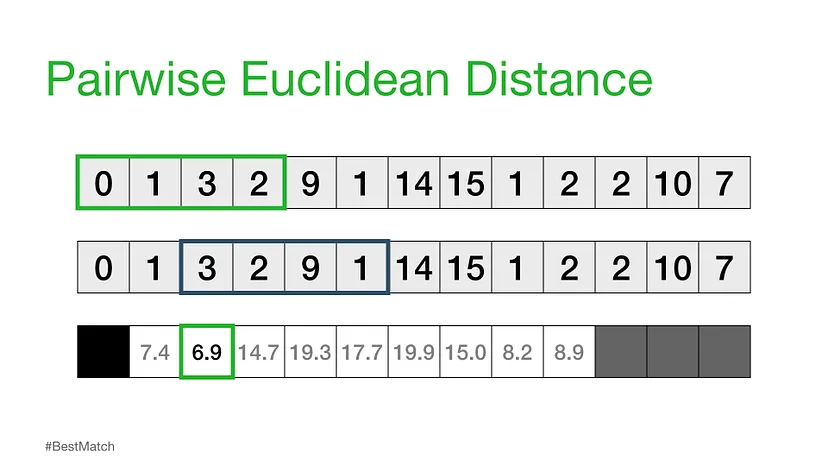
\includegraphics[width=0.8\linewidth,keepaspectratio]{timeseries5}

		{\tiny (Ref: Thomas J. Fan - Time Series EDA with STUMPY)}		
        \end{center}
	

\end{frame}


%%%%%%%%%%%%%%%%%%%%%%%%%%%%%%%%%%%%%%%%%%%%%%%%%%%%%%%%%%%%%%%%%%%%%%%%%%%%%%%%%%
\begin{frame}[fragile]\frametitle{Distance Matrix}

Collect as a Matrix, then find min of each row, make a column, thats Matrix Profile.
      \begin{center}
        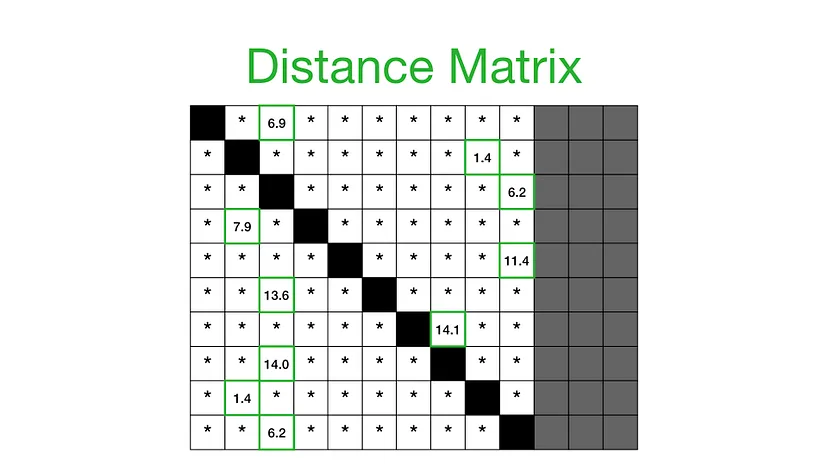
\includegraphics[width=0.8\linewidth,keepaspectratio]{timeseries6}

		{\tiny (Ref: Thomas J. Fan - Time Series EDA with STUMPY)}		
        \end{center}
	

\end{frame}

%%%%%%%%%%%%%%%%%%%%%%%%%%%%%%%%%%%%%%%%%%%%%%%%%%%%%%%%%%%%%%%%%%%%%%%%%%%%%%%%%%
\begin{frame}[fragile]\frametitle{Matrix Profile}

      \begin{center}

        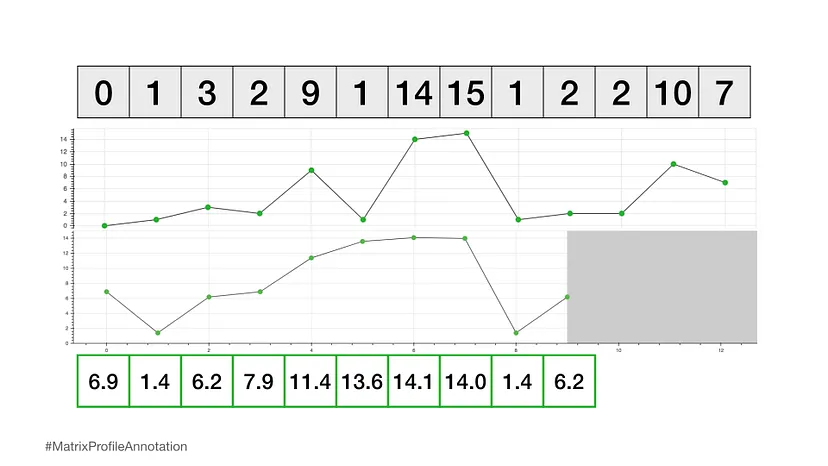
\includegraphics[width=0.8\linewidth,keepaspectratio]{timeseries7}

		{\tiny (Ref: Thomas J. Fan - Time Series EDA with STUMPY)}		
        \end{center}
	
Fully deterministic, only hyper-parameter is sub-sequence length
\end{frame}

%%%%%%%%%%%%%%%%%%%%%%%%%%%%%%%%%%%%%%%%%%%%%%%%%%%%%%%%%%%%%%%%%%%%%%%%%%%%%%%%%%
\begin{frame}[fragile]\frametitle{Z-normalization}
If you are interested in comparing only the shapes and not the amplitudes, then normalized both the sub-sequences before calculating distance.

      \begin{center}

        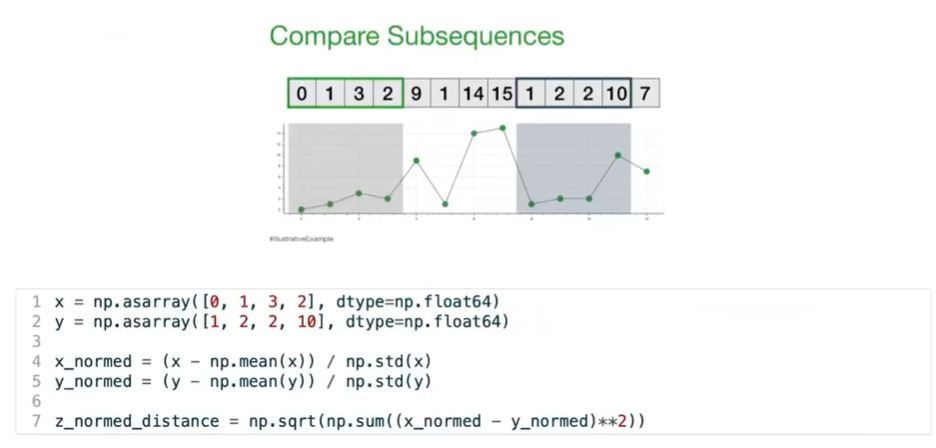
\includegraphics[width=0.8\linewidth,keepaspectratio]{timeseries8}

		{\tiny (Ref: Thomas J. Fan - Time Series EDA with STUMPY)}		
        \end{center}
	
\end{frame}

%%%%%%%%%%%%%%%%%%%%%%%%%%%%%%%%%%%%%%%%%%%%%%%%%%%%%%%%%%%%%%%%%%%%%%%%%%%%%%%%%%
\begin{frame}[fragile]\frametitle{Matrix Profile Fundamentals}
    \begin{itemize}
        \item Definition: Vector of distances between subsequences
        \item Components:
            \begin{itemize}
                \item Matrix Profile (series of distances of the closest neighbor). The  $i^{th}$   element  in  the  matrix  profile  $P$  indicates  the  Euclidean  distance  from subsequence $T_{i,m}$  to its nearest neighbor in time series $T$. However, it does not indicate the  location  of  that  nearest  neighbor.  This  information  is  recorded  in  a  companion data structure called the matrix profile index.
                \item Matrix Profile Index (series of indices of the closest neighbor)
            \end{itemize}
        \item Based on z-normalized Euclidean distance
    \end{itemize}
\begin{lstlisting}[language=Python]
[MP, MPindex] = computeMatrixProfile(T,m);        
[JMP, JMPindex] = computeMatrixProfileJoin(A,B,m); 
\end{lstlisting}

\end{frame}

%%%%%%%%%%%%%%%%%%%%%%%%%%%%%%%%%%%%%%%%%%%%%%%%%%%%%%%%%%%%%%%%%%%%%%%%%%%%%%%%%%
\begin{frame}[fragile]\frametitle{Distance Calculation}
    \begin{itemize}
        \item Z-normalization importance
        \item Distance measure:
            \begin{equation*}
            D(Q,T) = \sqrt{\sum_{i=1}^{m}(q_i - t_i)^2}
            \end{equation*}
    \end{itemize}
	
	
\end{frame}

%%%%%%%%%%%%%%%%%%%%%%%%%%%%%%%%%%%%%%%%%%%%%%%%%%%%%%%%%%%%%%%%%%%%%%%%%%%%%%%%%%
\begin{frame}[fragile]\frametitle{Sliding window approach}
	
      \begin{center}
        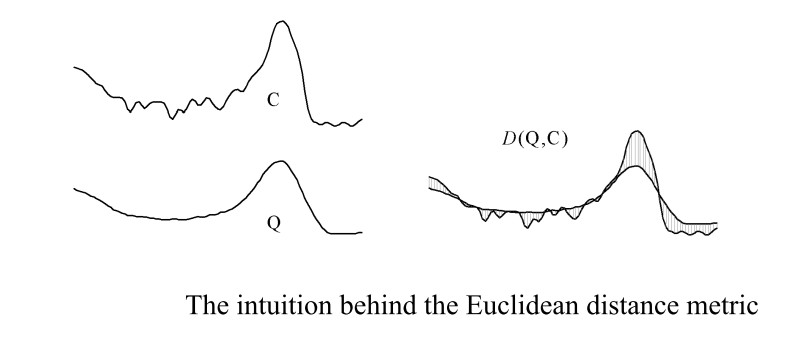
\includegraphics[width=0.8\linewidth,keepaspectratio]{intuition_distance}

        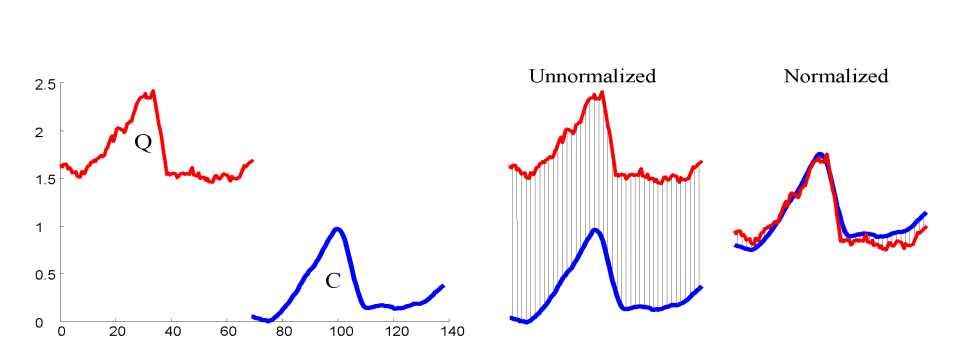
\includegraphics[width=0.8\linewidth,keepaspectratio]{normalized_ts}

		{\tiny (Ref: Mining Time Series Data - Chotirat Ann Ratanamahatana)}		
        \end{center}
	
\end{frame}


%%%%%%%%%%%%%%%%%%%%%%%%%%%%%%%%%%%%%%%%%%%%%%%%%%%%%%%%%%%%%%%%%%%%%%%%%%%%%%%%%%
\begin{frame}[fragile]\frametitle{STOMP Algorithm}
    \begin{itemize}
        \item Scalable Time series Ordered-search Matrix Profile
        \item Computational complexity: O(n²)
        \item Key optimization techniques:
            \begin{itemize}
                \item Dot product calculation
                \item Distance calculation
            \end{itemize}
    \end{itemize}
\end{frame}

%%%%%%%%%%%%%%%%%%%%%%%%%%%%%%%%%%%%%%%%%%%%%%%%%%%%%%%%%%%%%%%%%%%%%%%%%%%%%%%%%%
\begin{frame}[fragile]\frametitle{Motif Discovery}
    \begin{itemize}
        \item Definition: Repeated patterns in time series
        \item Detection using Matrix Profile:
            \begin{itemize}
                \item Lowest points in profile
                \item Chain detection
            \end{itemize}
        \item Significance assessment
    \end{itemize}
	

\end{frame}

%%%%%%%%%%%%%%%%%%%%%%%%%%%%%%%%%%%%%%%%%%%%%%%%%%%%%%%%%%%%%%%%%%%%%%%%%%%%%%%%%%
\begin{frame}[fragile]\frametitle{Discord Detection}
    \begin{itemize}
        \item Definition: Anomalous subsequences
        \item Identification method:
            \begin{itemize}
                \item Highest points in profile
                \item Contextual analysis
            \end{itemize}
        \item Applications in anomaly detection
    \end{itemize}
\end{frame}